\part{Linear-Algebra}
\lecture{Linear Algebra}{Linear-Algebra}
\section{Linear Algebra}

\title{Ordinary Differential Equations}
\subtitle{Introduction to Linear Algebra}
\date{13 October 2013}

\begin{frame}
  \titlepage
\end{frame}

\begin{frame}
  \frametitle{Outline}
  \tableofcontents[ currentsection ]
\end{frame}


\subsection{Linear Algebra}


\begin{frame}
  \frametitle{Linear Algebra}


  \begin{eqnarray*}
    3x + 2y & = & 7 \\
    4x - y & = & 1
  \end{eqnarray*}

  \uncover<2->
  {
    Alternate representation:
    \begin{eqnarray*}
      \arrayTwo{3}{2}{4}{-1} \vecTwo{x}{y} & = & \vecTwo{7}{1}.
    \end{eqnarray*}

    A matrix is an array of numbers arranged in rows and columns.

    A column vector is a matrix with one column.

  }


\end{frame}


\begin{frame}
  \frametitle{Matrix Addition/Subtraction}

  If two matrices have the same number of rows and columns you add the
  two matrices by adding/subtracting them entry by entry.

  \begin{eqnarray*}
    \arrayTwo{3}{-1}{2}{4} + \arrayTwo{7}{6}{2}{1} & = & \arrayTwo{10}{5}{4}{5}
  \end{eqnarray*}

\end{frame}


\begin{frame}
  \frametitle{Scalar Multiplication}

  Multiply every entry in the matrix by the same number.

  \begin{eqnarray*}
    4 \arrayTwo{3}{-1}{2}{4} & = & \arrayTwo{12}{-4}{8}{16}
  \end{eqnarray*}


\end{frame}


\begin{frame}
  \frametitle{Transpose}

  Switch the rows and the columns:
  \begin{eqnarray*}
    \arrayTwo{\redText{2}}{\redText{7}}{\blueText{4}}{\blueText{6}}^T & = & 
      \arrayTwo{\redText{2}}{\blueText{4}}{\redText{7}}{\blueText{6}} \\
    \left[
    \begin{array}{r}
      1 \\ 7 \\ 3 \\ 2
    \end{array}
    \right]^T & = & 
    \left[
    \begin{array}{rrrr}
      1 & 7 & 3 & 2
    \end{array}
    \right]
  \end{eqnarray*}

\end{frame}


\begin{frame}
  \frametitle{Matrix Multiplication}

  \begin{eqnarray*}
    \left[
    \begin{array}{rrrr}
      a_{11} & a_{12} & \cdots & a_{1m} \\
      a_{21} & a_{22} & \cdots & a_{2m} \\
      \vdots &       & \ddots & \vdots \\ 
      \color{red}{\mathbf{a_{i1}}} & \color{red}{\mathbf{a_{i2}}} & \color{red}{\mathbf{\cdots}} & \color{red}{\mathbf{a_{im}}} \\ 
      \vdots &       & \ddots & \vdots \\
      a_{n1} & a_{n2} & \cdots & a_{nm}
    \end{array}
  \right] \cdot
    \left[
    \begin{array}{rrrrr}
      b_{11}  & \cdots & \color{blue}{\mathbf{b_{1j}}}  & \cdots  & b_{1k} \\
      b_{21}  & \cdots & \color{blue}{\mathbf{b_{2j}}}  & \cdots  & b_{2k} \\
      \vdots &        & \color{blue}{\mathbf{\vdots}} & \vdots & \vdots \\
      b_{m1}  & \cdots & \color{blue}{\mathbf{b_{mj}}}  & \cdots & b_{mk}
    \end{array}
  \right]  =  \\
    \left[
    \begin{array}{rrrrr}
      * & \cdots & * & \cdots  &  * \\
      *  & \cdots & *  & \cdots  &  * \\
      \vdots &        & c_{ij} & \vdots & \vdots \\
      * & \cdots & *  & \cdots & *
    \end{array}
  \right]
  \end{eqnarray*}

  Entry in row i and column j is 
  \begin{eqnarray*}
    c_{ij} & = & \redText{a_{i1}}\blueText{b_{1j}} + \redText{a_{i2}}\blueText{b_{2j}} + \cdots + \redText{a_{im}}\blueText{b_{mj}}
  \end{eqnarray*}

\end{frame}


\begin{frame}
  \frametitle{Matrix Multiplication}

  \begin{eqnarray*}
    \left[
    \begin{array}{rrrr}
      a_{11} & a_{12} & \cdots & a_{1m} \\
      a_{21} & a_{22} & \cdots & a_{2m} \\
      \vdots &       & \ddots & \vdots \\ \hline
      \color{red}{\mathbf{a_{i1}}} & \color{red}{\mathbf{a_{i2}}} & \color{red}{\mathbf{\cdots}} & \color{red}{\mathbf{a_{im}}} \\ \hline
      \vdots &       & \ddots & \vdots \\
      a_{n1} & a_{n2} & \cdots & a_{nm}
    \end{array}
  \right] \cdot
    \left[
    \begin{array}{rr|r|rr}
      b_{11}  & \cdots & \color{blue}{\mathbf{b_{1j}}}  & \cdots  & b_{1k} \\
      b_{21}  & \cdots & \color{blue}{\mathbf{b_{2j}}}  & \cdots  & b_{2k} \\
      \vdots &        & \color{blue}{\mathbf{\vdots}} & \vdots & \vdots \\
      b_{m1}  & \cdots & \color{blue}{\mathbf{b_{mj}}}  & \cdots & b_{mk}
    \end{array}
  \right]  =  \\
    \left[
    \begin{array}{rrrrr}
      * & \cdots & * & \cdots  &  * \\
      *  & \cdots & *  & \cdots  &  * \\
      \vdots &        & c_{ij} & \vdots & \vdots \\
      * & \cdots & *  & \cdots & *
    \end{array}
  \right]
  \end{eqnarray*}

  Entry in row i and column j is 
  \begin{eqnarray*}
    c_{ij} & = & \redText{a_{i1}}\blueText{b_{1j}} + \redText{a_{i2}}\blueText{b_{2j}} + \cdots + \redText{a_{im}}\blueText{b_{mj}}
  \end{eqnarray*}

\end{frame}


\begin{frame}
  \frametitle{Example}

  \begin{eqnarray*}
    \arrayTwo{\redText{2}}{\redText{7}}{4}{6} \cdot \arrayTwo{\blueText{2}}{1}{\blueText{-2}}{1} & = & 
    \arrayTwo{\fuchsiaText{-10}}{9}{-4}{10} \\
    \left[
      \begin{array}{rrr}
        2 & 3 & 1 \\ -1 & 2 & 1
      \end{array}
    \right] \cdot
    \left[
      \begin{array}{r}
        1 \\ 2 \\ 3
      \end{array}
    \right]
    & = & 
    \vecTwo{11}{6}
  \end{eqnarray*}

\end{frame}

\iftoggle{clicker}{%
\begin{frame}
  \frametitle{Clicker Quiz}
    
      \ifnum\value{clickerQuiz}=1{%

        \vfill

        Determine the value of 
        \begin{eqnarray*}
          \arrayTwo{2}{-1}{3}{1} \cdot \vecTwo{1}{3}
        \end{eqnarray*}
        
        \begin{eqnarray*}
          \begin{array}{lcl@{\hspace{3em}}lcl}
            A: &  = & \vecTwo{6}{-1} &
            B: &  = & \vecTwo{1}{4} \\ [12pt]
            C: &  = & \vecTwo{1}{0} &
            D: &  = & \vecTwo{-1}{6}
          \end{array}
        \end{eqnarray*}

          \vfill

     }\fi

     \ifnum\value{clickerQuiz}=2{%

        \vfill

        Determine the value of 
        \begin{eqnarray*}
          \arrayTwo{1}{4}{2}{-1} \cdot \vecTwo{1}{3}
        \end{eqnarray*}
        
        \begin{eqnarray*}
          \begin{array}{lcl@{\hspace{3em}}lcl}
            A: &  = & \vecTwo{7}{5} &
            B: &  = & \vecTwo{5}{1} \\ [12pt]
            C: &  = & \vecTwo{13}{-1} &
            D: &  = & \vecTwo{5}{3}
          \end{array}
        \end{eqnarray*}

          \vfill

     }\fi

      \ifnum\value{clickerQuiz}=3{%
        \vfill

        \begin{columns}
          \column{.5\textwidth}
          Determine the value of
          \begin{eqnarray*}
            \arrayTwo{1}{2}{4}{-3} \cdot \vecTwo{-1}{1}
          \end{eqnarray*}
          \column{.5\textwidth}
          \begin{eqnarray*}
            \begin{array}{lcl}
              A: &  = &  [\begin{array}{rr}  1 & -7\end{array}]  \\ [12pt] 
              B: &  = & [\begin{array}{rr}  3 & -5\end{array}] \\ [12pt]
              C: &  = & \vecTwo{1}{-7} \\ [12pt] 
              D: &  = & \vecTwo{3}{-5}\\ %[12pt]
              % E: & = & \arrayTwo{-1}{2}{-4}{3}
            \end{array}
          \end{eqnarray*}
        \end{columns}
       \vfill

     }\fi

    \vfill
    \vfill
    \vfill

\end{frame}

}

\subsection{Matrices to Know}

\begin{frame}
  \frametitle{Matrices to Know}

  A diagonal matrix is in the form
  \begin{eqnarray*}
    \left[
      \begin{array}{rrrr}
        a_{11} & 0 & \\
        0 & a_{22} & 0 \\
        & & \ddots & 0\\
        & & 0 & a_{nn}
      \end{array}
    \right]
  \end{eqnarray*}

  Special case, the identity matrix:
  \begin{eqnarray*}
    I_n & = & 
    \left[
      \begin{array}{rrrr}
        1 & 0 & \\
        0 & 1 & 0 \\
        & & \ddots & 0 \\
        & & 0 & 1
      \end{array}
    \right]
  \end{eqnarray*}

\end{frame}

\begin{frame}
  \frametitle{Example}

  Special case, the identity matrix:
  \begin{eqnarray*}
    I_3 & = & 
    \left[
      \begin{array}{rrr}
        1 & 0 & 0\\
        0 & 1 & 0 \\
        0 & 0 & 1
      \end{array}
    \right]
  \end{eqnarray*}

  Note:
  \begin{eqnarray*}
    \left[
      \begin{array}{rrr}
        1 & 0 & 0 \\
        0 & 1 & 0 \\
        0 & 0 & 1
      \end{array}
    \right] \cdot
       \left[
      \begin{array}{rrr}
        3 & 4 & 2 \\
        -5 & 6 & 7 \\
        8 & 7 & 3
      \end{array}
    \right] & = & 
       \left[
      \begin{array}{rrr}
        3 & 4 & 2 \\
        -5 & 6 & 7 \\
        8 & 7 & 3
      \end{array}
    \right] 
  \end{eqnarray*}

  In general $I_n\cdot A = A$.

\end{frame}


\subsection{Vector Operations}

\begin{frame}
  \frametitle{Vector Operations}

  If
  \begin{eqnarray*}
    \vec{x} & = & 
    \left[
    \begin{array}{r}
      x_1 \\ x_2 \\ \vdots \\ x_n
    \end{array}
    \right]
  \end{eqnarray*}
  then
  \begin{eqnarray*}
    \left[
      \begin{array}{rrrr}
        x_1 & x_2 & \cdots & x_n
      \end{array}
    \right] \cdot
    \left[
      \begin{array}{r}
        x_1 \\ x_2 \\ \vdots \\ x_n
      \end{array}
    \right] & = & 
    x_1^2 + x_2^2 + \cdots + x_n^2
  \end{eqnarray*}

\end{frame}


\begin{frame}
  \frametitle{The Dot Product}

  The dot product:
  \begin{eqnarray*}
    \vec{x} \cdot \vec{y} & = & \vec{x}^T \vec{y} 
  \end{eqnarray*}

  The norm:
  \begin{eqnarray*}
    \| \vec{x} \| & = & \sqrt{\vec{x}^T \vec{x}}
  \end{eqnarray*}

\end{frame}

\subsection{Orthogonality}

\begin{frame}
  \frametitle{Orthogonality}

  \begin{eqnarray*}
    \vec{x} & = & \vecTwo{1}{0} \\
    \vec{y} & = & \vecTwo{0}{1} \\
    \vec{x}\cdot\vec{y} & = & 0
  \end{eqnarray*}

  In general,
  \begin{eqnarray*}
    \vec{u}\cdot\vec{v} & = & \| \vec{u} \| \| \vec{v} \| \cos(\theta)
  \end{eqnarray*}

  Definition, if $\vec{u}\cdot\vec{v}=0$ then the vectors are \textbf{orthogonal}.

\end{frame}


\begin{frame}
  \frametitle{Example}

  \begin{eqnarray*}
    \vec{x} & = & 
    \left[
      \begin{array}{r}
        2 \\ 4 \\ -1
      \end{array} \right] \\
      \| \vec{x} \| & = & \sqrt{2^2 + 4^2 + (-1)^2} \\
      & = & \sqrt{21}
  \end{eqnarray*}

\end{frame}




\subsection{Differentiation}

\begin{frame}
  \frametitle{Differentiation}

  The derivative of a matrix is the derivative of each of its elements.
  \begin{eqnarray*}
    \frac{d}{dt} \arrayTwo{3t^{-1}}{\sin(t)}{\sqrt{t+1}}{\tan(t)} & = & 
    \arrayTwo{-3t^{-2}}{\cos(t)}{\half\lp t+1\rp^{-\half}}{\sec^2(t)}
  \end{eqnarray*}

\end{frame}

\begin{frame}
  \frametitle{Why bother?}

  Suppose that
  \begin{eqnarray*}
    \frac{d}{dt} x & = & 3x + 2y \\
    \frac{d}{dt} y & = & -2 x + 4 y
  \end{eqnarray*}

  Another way to express the system:
  \begin{eqnarray*}
    \frac{d}{dt} \vecTwo{x}{y} & = & \arrayTwo{3}{2}{-2}{4} \vecTwo{x}{y}
  \end{eqnarray*}

\end{frame}


\iftoggle{clicker}{%
\begin{frame}
  \frametitle{Clicker Quiz}
    
      \ifnum\value{clickerQuiz}=1{%

        \vfill

        Express the system
        \begin{eqnarray*}
          \frac{d}{dt} x & = & -x + 2y \\
          \frac{d}{dt} y & = & 3x + y
        \end{eqnarray*}
        in matrix/vector form.

        
        \begin{eqnarray*}
          A: \frac{d}{dt} \vecTwo{x}{y} & = & \arrayTwo{-1}{3}{2}{1} \vecTwo{x}{y} \\ [12pt]
          B: \frac{d}{dt} \vecTwo{x}{y} & = & \arrayTwo{-1}{2}{3}{1} \vecTwo{x}{y} 
        \end{eqnarray*}

          \vfill

     }\fi

     \ifnum\value{clickerQuiz}=2{%

        \vfill

        \vfill

        Express the system
        \begin{eqnarray*}
          \frac{d}{dt} x & = & 4x + y \\
          \frac{d}{dt} y & = & -x + 3 y
        \end{eqnarray*}
        in matrix/vector form.

        
        \begin{eqnarray*}
          A: \frac{d}{dt} \vecTwo{x}{y} & = & \arrayTwo{4}{1}{-1}{3} \vecTwo{x}{y} \\ [12pt]
          B: \frac{d}{dt} \vecTwo{x}{y} & = & \arrayTwo{4}{-1}{1}{3} \vecTwo{x}{y} 
        \end{eqnarray*}

          \vfill

     }\fi

      \ifnum\value{clickerQuiz}=3{%
        \vfill

        Express the system
        \begin{eqnarray*}
          \frac{d}{dt} x & = & 5x + 2y \\
          \frac{d}{dt} y & = & 3x - 4y
        \end{eqnarray*}
        in matrix/vector form.


        \begin{eqnarray*}
          A: \frac{d}{dt} \vecTwo{x}{y} & = & \arrayTwo{5}{2}{-4}{3} \vecTwo{x}{y} \\ [12pt]
          B: \frac{d}{dt} \vecTwo{x}{y} & = & \arrayTwo{5}{2}{3}{-4} \vecTwo{x}{y} \\ [12pt]
          C: \frac{d}{dt} \vecTwo{x}{y} & = & \arrayTwo{5}{3}{2}{-4} \vecTwo{x}{y} 
        \end{eqnarray*}

          \vfill

     }\fi

    \vfill
    \vfill
    \vfill

\end{frame}

}


\begin{frame}
  \frametitle{Double Tank Problem}

  \begin{columns}
    \column{.35\textwidth}
    {\includegraphics[width=1.5\textwidth]{img/introLinearAlgebraTankProblem}}    

    \column{.65\textwidth}

    Define:

    $x(t)$ is the \redText{amount} of salt in tank 1 (in \blueText{g}).

    $y(t)$ is the \redText{amount} of salt in tank 2 (in \blueText{g}).
    \vspace{3cm}
  \end{columns}
\end{frame}

\begin{frame}
  \frametitle{Double Tank Problem}

    $x(t)$ is the amount of salt in tank 1 (in g), and $y(t)$ is the amount of salt in tank 2 (in g).

    \vfill

    The rates of change for the amounts (in g) can now be expressed as
    the following for tank one:
    \begin{tabular}{l@{\hspace{2em}}l}
      rate in, tank 1:  & 4 l/min $\times$ 4 g/l + $\frac{y~g}{100~l} \times$ 2 l/min,\\
      rate out, tank 1: & 6 l/min $\times \frac{x~g}{200~l}$,\\
    \end{tabular}

    \vfill

    The rates of change for the amounts (in g) can now be expressed as
    the following for tank two:
    \begin{tabular}{l@{\hspace{2em}}l}
      rate in, tank 2:  & 6 l/min $\times \frac{x~g}{200~l}$,\\
      rate out, tank 2: & 4 l/min $\times \frac{y~g}{100~l}$ + 2 l/min $\times \frac{y~g}{100~l}.$
    \end{tabular}

    \vfill


\end{frame}

\begin{frame}{System of Differential Equations}
  
  This leads to a \textit{system} of differential equations,
    \begin{eqnarray*}
      \dot{x} & = & 16 + \frac{2y}{100} - \frac{6x}{200}, \\
      \dot{y} & = &  \frac{6x}{200} - \frac{6y}{100}. \\
    \end{eqnarray*}

    \vfill

\end{frame}

\begin{frame}
  \frametitle{Double Tank Problem}

    $x$ is the amount of salt in tank 1 (in g), and $y$ is the amount of salt in tank 2 (in g).

    From the system of differential equations,
    \begin{eqnarray*}
      \dot{x} & = & 16 - \frac{6x}{200} + \frac{2y}{100}, \\
      \dot{y} & = &  \frac{6x}{200} - \frac{6y}{100}, \\
    \end{eqnarray*}
    we can express them in matrix/vector form,
    \begin{eqnarray*}
      \frac{d}{dt} \left[
        \begin{array}{l}
          x \\ y
        \end{array}
      \right]
      & = & 
      \left[
        \begin{array}{ll}
          \frac{-6}{200} & \frac{2}{100}  \\ 
          \frac{6}{200}   & \frac{-6}{100} 
        \end{array}
      \right]
      \left[
        \begin{array}{l}
          x \\ y
        \end{array}
        \right]
        +
        \left[
        \begin{array}{l}
          16 \\ 0
        \end{array}
        \right]
    \end{eqnarray*}


\end{frame}




% LocalWords:  Clarkson pausesection hideothersubsections
